\begin{appendices}
\addcontentsline{toc}{section}{Appendix}

\section{Additional tables}

\begin{table}[H]
    \centering
    \scriptsize
    \renewcommand{\arraystretch}{1.25}
    \setlength{\tabcolsep}{3pt}
    \begin{tabular}{>{\raggedright\arraybackslash}p{2.6cm}>{\raggedright\arraybackslash}p{2.5cm}>{\raggedright\arraybackslash}p{3.9cm}>{\raggedright\arraybackslash}p{1.3cm}>{\raggedright\arraybackslash}p{1.1cm}>{\raggedright\arraybackslash}p{3.7cm}}
\hline
algorithm & technique & complexity & slope real & slope adv. & largest run (real / adv.) \\
\hline
naive search & brute force & $O(nm)$ & 1.03 & 1.03 & 1.6 ms / 39.4 ms, $n = 29903$ \\
KMP & string & $O(n + m)$ & 1.00 & 1.00 & 1.4 ms / 2.0 ms, $n = 29903$ \\
Z-function & string & $O(n + m)$ & 1.01 & 1.00 & 3.4 ms / 4.8 ms, $n = 29903$ \\
LCS rows, Python & DP & $O(nm)$ time, $O(m)$ space & 2.08 & -- & 438.5 ms, $n = 3000$ \\
LCS rows, numpy & DP & $O(nm)$ time, $O(m)$ space & 1.86 & -- & 1.63 s, $n = 29903$ \\
Hirschberg & D\&C + DP & $O(nm)$ time, $O(n + m)$ space & 1.78 & -- & 3.80 s, $n = 29903$ \\
ORF selection & greedy & $O(n + c \log c)$ vs $O(2^c)$ & 1.04 (scan) & -- & exhaustive 38.6 ms, $c = 16$ \\
protein localisation & backtracking & $O(6^k)$ worst, pruned & -- & -- & 108 vs 995328 nodes, $k = 10$ \\
motif search & branch and bound & $O(4^k n)$ worst, pruned & -- & -- & 6383 vs 85695 nodes, $k = 8$ \\
centre expansion & brute force & $O(n^2)$ & 1.05 & 2.00 & 8.3 ms / 364.8 ms \\
Manacher & string & $O(n)$ & 1.04 & 1.04 & 10.6 ms / 1.6 ms \\
\hline
\end{tabular}
    \caption{Theoretical complexity against the measured log-log slope of running time versus input size. Timings from one run of the notebook on a laptop.}
    \label{tab:complexity}
\end{table}

\begin{table}[H]
    \centering
    \scriptsize
    \begin{tabular}{lrrrrrrr}
\hline
protein & length & start & end & frame & matched & nodes & pruned \\
\hline
QHD43415\_1 & 180 & 265 & 805 & 1 & 180/180 & 41 & 32 \\
QHD43415\_2 & 638 & 805 & 2719 & 1 & 638/638 & 86 & 65 \\
QHD43415\_3 & 1945 & 2719 & 8554 & 1 & 1945/1945 & 76 & 56 \\
QHD43415\_4 & 500 & 8554 & 10054 & 1 & 500/500 & 41 & 27 \\
QHD43415\_5 & 306 & 10054 & 10972 & 1 & 306/306 & 97 & 66 \\
QHD43415\_6 & 290 & 10972 & 11842 & 1 & 290/290 & 140 & 103 \\
QHD43415\_7 & 83 & 11842 & 12091 & 1 & 83/83 & 56 & 31 \\
QHD43415\_8 & 198 & 12091 & 12685 & 1 & 198/198 & 86 & 64 \\
QHD43415\_9 & 113 & 12685 & 13024 & 1 & 113/113 & 42 & 30 \\
QHD43415\_10 & 139 & 13024 & 13441 & 1 & 139/139 & 68 & 45 \\
QHD43415\_11 & 932 & 13441 & 16237 & 1 & 9/932 & 90 & 58 \\
QHD43415\_12 & 601 & 16236 & 18039 & 0 & 601/601 & 102 & 76 \\
QHD43415\_13 & 527 & 18039 & 19620 & 0 & 527/527 & 42 & 26 \\
QHD43415\_14 & 346 & 19620 & 20658 & 0 & 346/346 & 142 & 87 \\
QHD43415\_15 & 298 & 20658 & 21552 & 0 & 298/298 & 143 & 93 \\
QHD43416 & 1273 & 21562 & 25381 & 1 & 1273/1273 & 25 & 17 \\
QHD43417 & 275 & 25392 & 26217 & 0 & 275/275 & 26 & 18 \\
QHD43418 & 75 & 26244 & 26469 & 0 & 75/75 & 29 & 21 \\
QHD43419 & 222 & 26522 & 27188 & 2 & 222/222 & 37 & 26 \\
QHD43420 & 61 & 27201 & 27384 & 0 & 61/61 & 23 & 15 \\
QHD43421 & 121 & 27393 & 27756 & 0 & 121/121 & 23 & 15 \\
QHD43422 & 121 & 27893 & 28256 & 2 & 121/121 & 19 & 12 \\
QHD43423 & 419 & 28273 & 29530 & 1 & 419/419 & 31 & 19 \\
QHI42199 & 38 & 29557 & 29671 & 1 & 38/38 & 22 & 13 \\
\hline
\end{tabular}
    \caption{Proteins located by backtracking with $k = 6$ amino acids (0-based genome positions). Matched is the number of leading amino acids reproduced by translating the genome from the located start.}
    \label{tab:proteins}
\end{table}

\begin{table}[H]
    \centering
    \small
    \begin{tabular}{rrrrl}
\hline
start & end & frame & codons & known gene overlap \\
\hline
265 & 13483 & 1 & 4405 & ORF1ab (62\%) \\
13767 & 21555 & 0 & 2595 & ORF1ab (37\%) \\
21562 & 25384 & 1 & 1273 & S (100\%) \\
25392 & 26220 & 0 & 275 & - \\
26522 & 27191 & 2 & 222 & M (100\%) \\
27393 & 27759 & 0 & 121 & - \\
27893 & 28259 & 2 & 121 & - \\
28273 & 29533 & 1 & 419 & - \\
\hline
\end{tabular}
    \caption{ORFs selected by greedy activity selection among candidates with at least 100 codons (0-based positions).}
    \label{tab:orfs}
\end{table}

\begin{table}[H]
    \centering
    \small
    \begin{tabular}{rrlrrr}
\hline
$k$ & $d$ & best motif & count & exhaustive nodes & B\&B nodes \\
\hline
5 & 1 & TTTTT & 1241 & 1365 & 263 \\
6 & 1 & TTTTTT & 418 & 5461 & 907 \\
7 & 1 & TGTTGTT & 193 & 21836 & 2252 \\
8 & 1 & TGTTGTTA & 75 & 85695 & 6383 \\
10 & 1 & AAAAGAAAAA & 33 & -- & 15575 \\
12 & 1 & AAAAAAAAAAAA & 24 & -- & 22445 \\
\hline
\end{tabular}
    \caption{Most frequent $k$-mer with up to one mismatch in the Wuhan genome.}
    \label{tab:motif}
\end{table}

\begin{table}[H]
    \centering
    \small
    \begin{tabular}{lrlrrr}
\hline
gene & length & longest palindrome & start & end & length \\
\hline
M & 669 & \texttt{CTAAAGAAATC} & 493 & 504 & 11 \\
S & 3822 & \texttt{GAATTTGTGTTTAAG} & 570 & 585 & 15 \\
orf1ab & 21290 & \texttt{CTCAATGACTTCAGTAACTC} & 9711 & 9731 & 20 \\
\hline
\end{tabular}
    \caption{Longest palindrome per gene (0-based positions inside the gene).}
    \label{tab:palindromes}
\end{table}

\section{Additional figures}

\begin{figure}[H]
    \centering
    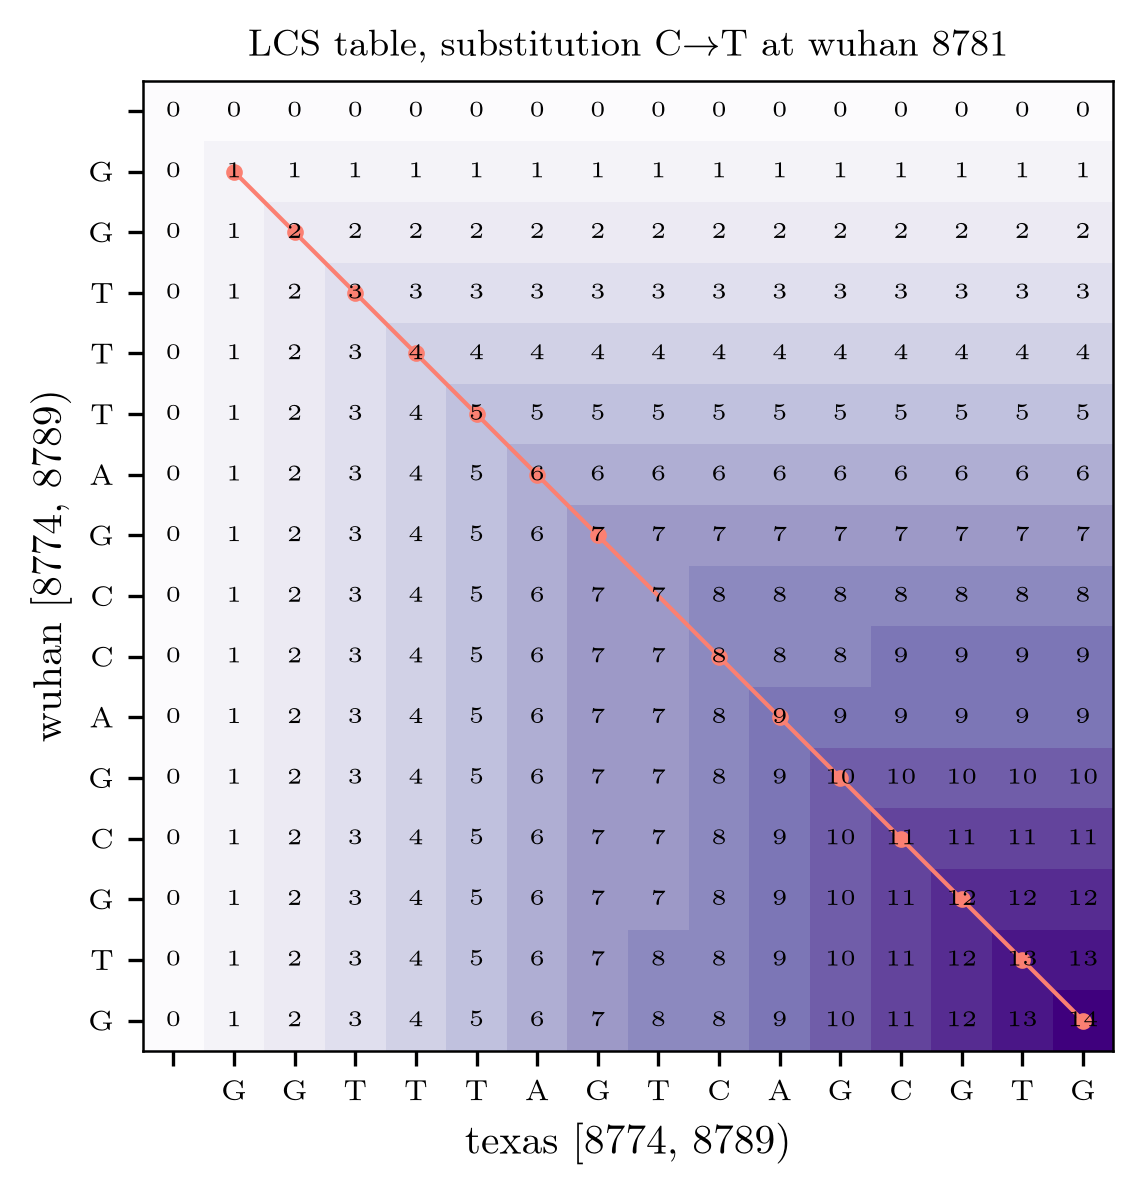
\includegraphics[width=0.48\textwidth]{fig_lcs_matrix}
    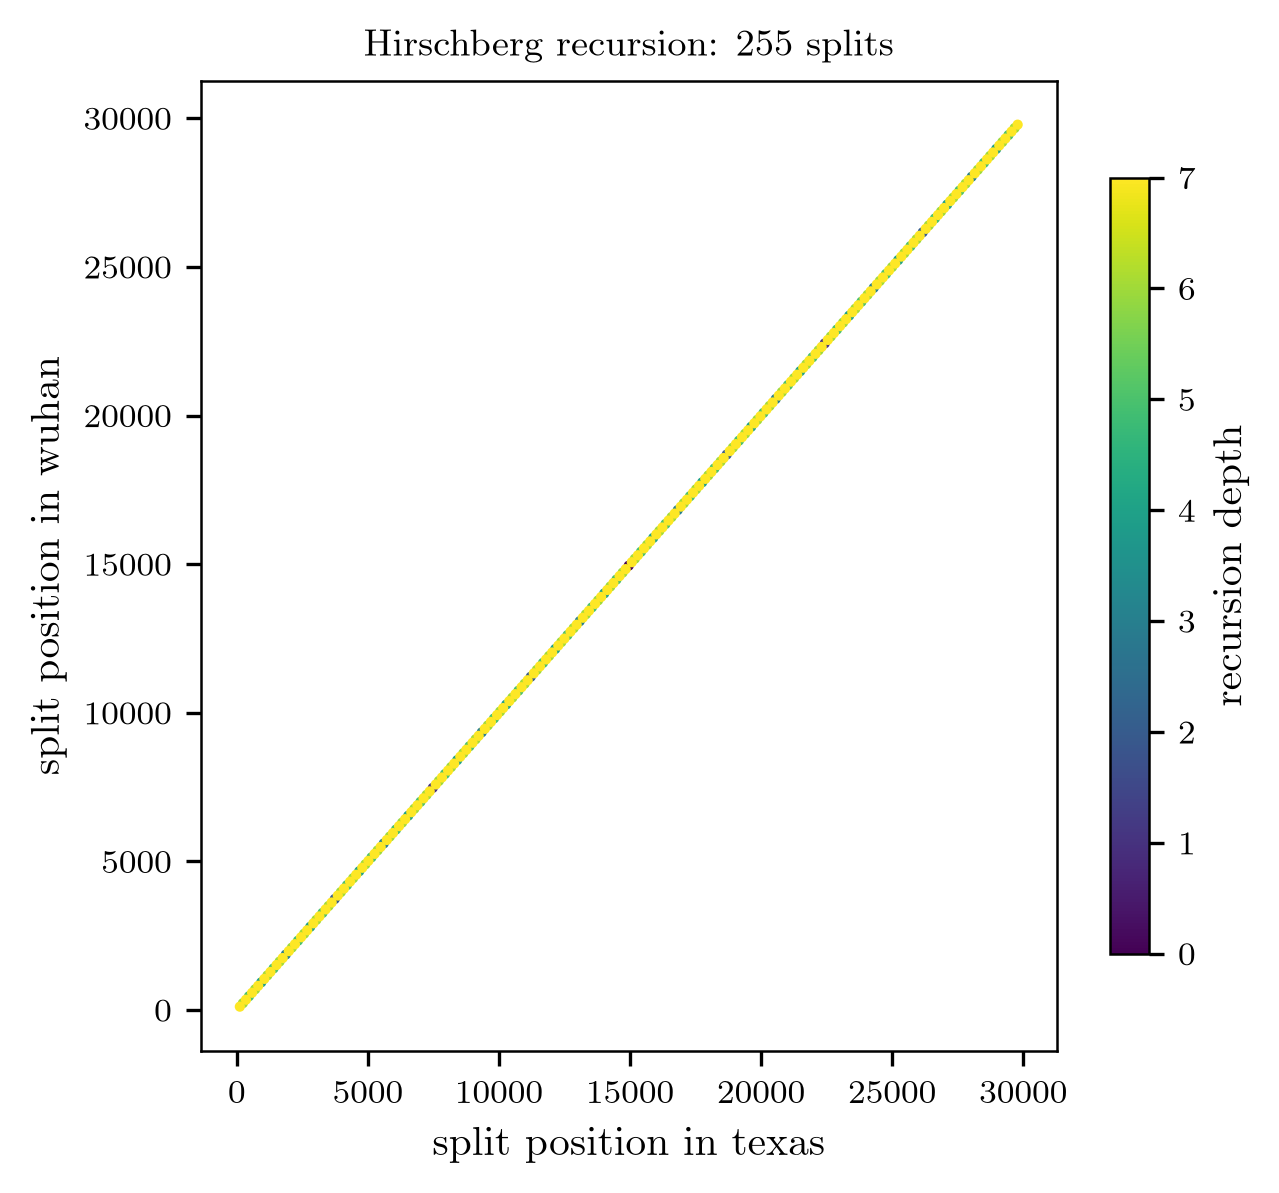
\includegraphics[width=0.48\textwidth]{fig_hirschberg_splits}
    \caption{Left: LCS table and traceback on a 15-symbol window around the first substitution. Right: the split points chosen by Hirschberg's recursion on the two genomes, coloured by depth.}
    \label{fig:splits}
\end{figure}

\begin{figure}[H]
    \centering
    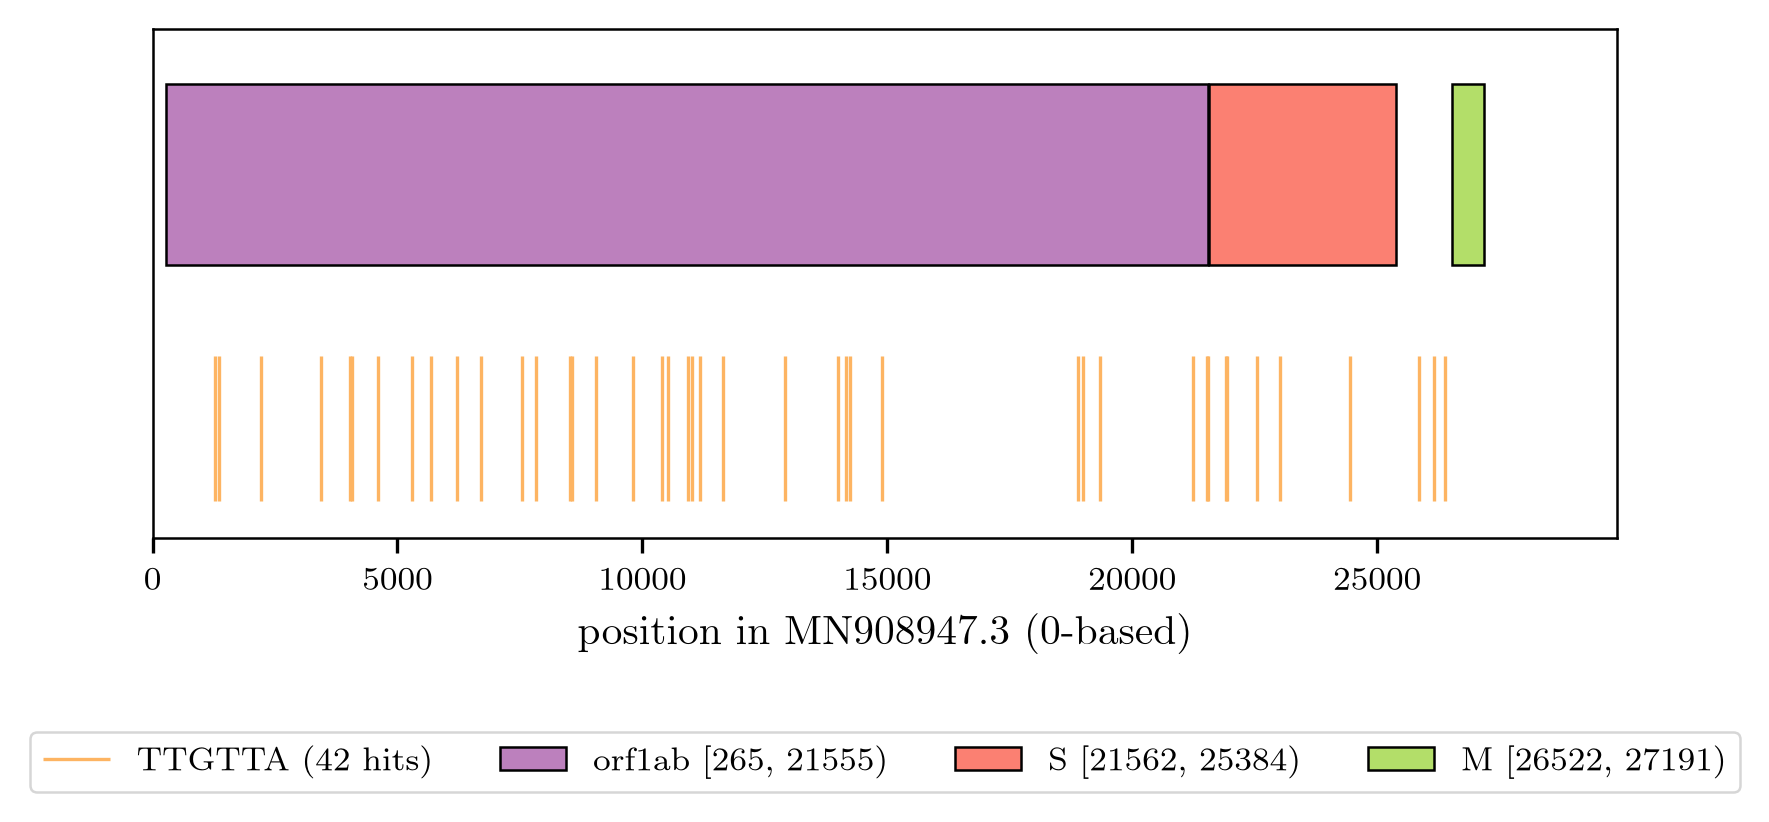
\includegraphics[width=0.85\textwidth]{fig_gene_map}
    \caption{Genes located by pattern search in the Wuhan genome and the occurrences of the most frequent 6-mer.}
    \label{fig:gene_map}
\end{figure}

\begin{figure}[H]
    \centering
    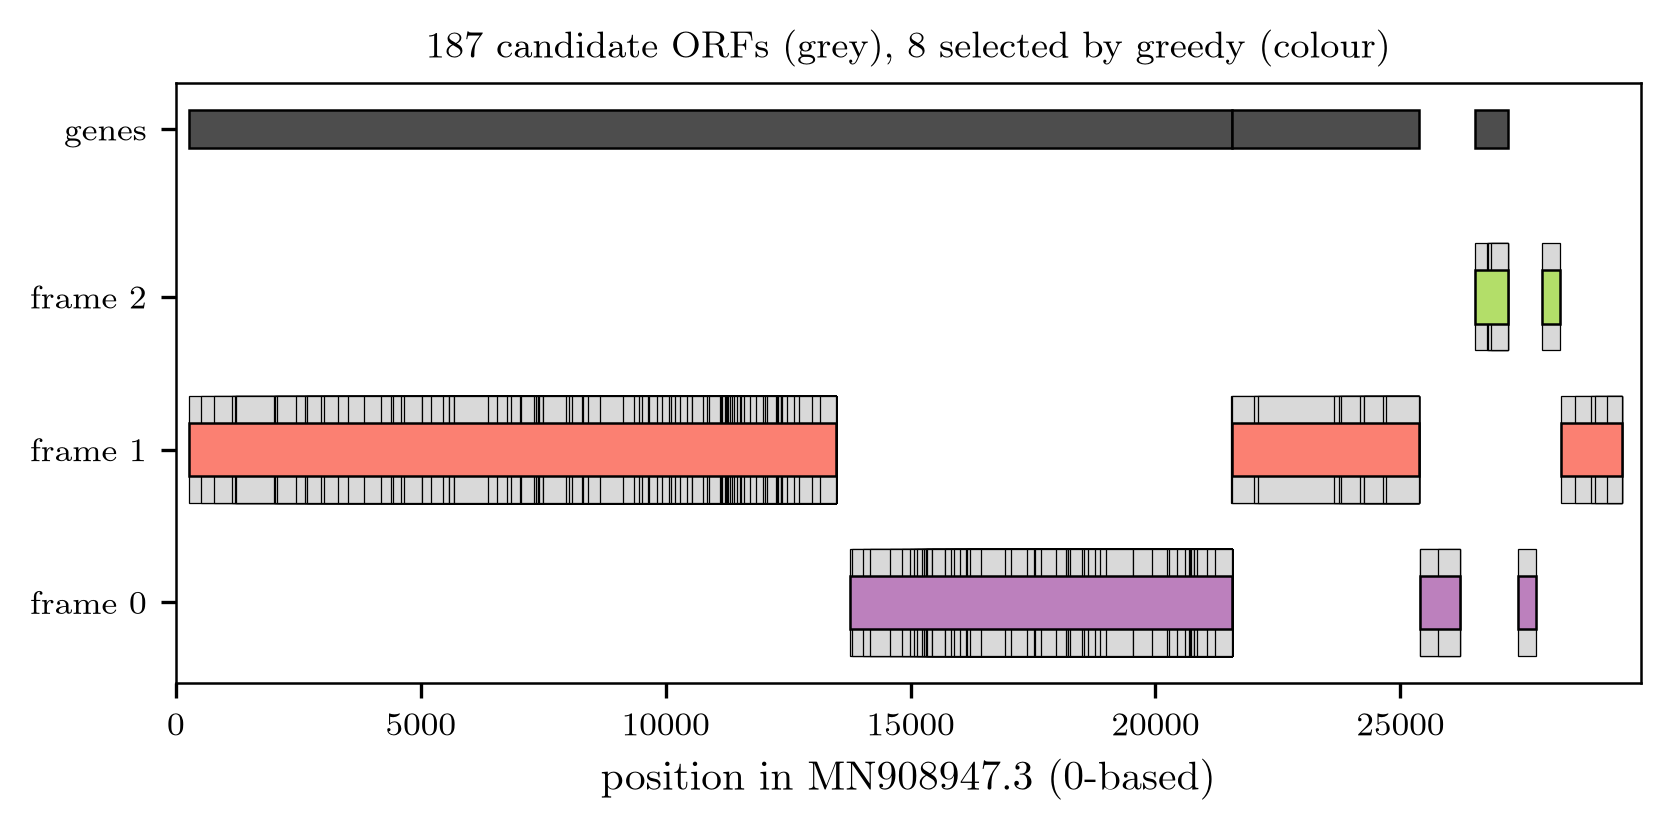
\includegraphics[width=0.85\textwidth]{fig_orf_map}
    \caption{Candidate ORFs per reading frame (grey) and the greedy selection (colour) against the known genes.}
    \label{fig:orf}
\end{figure}

\begin{figure}[H]
    \centering
    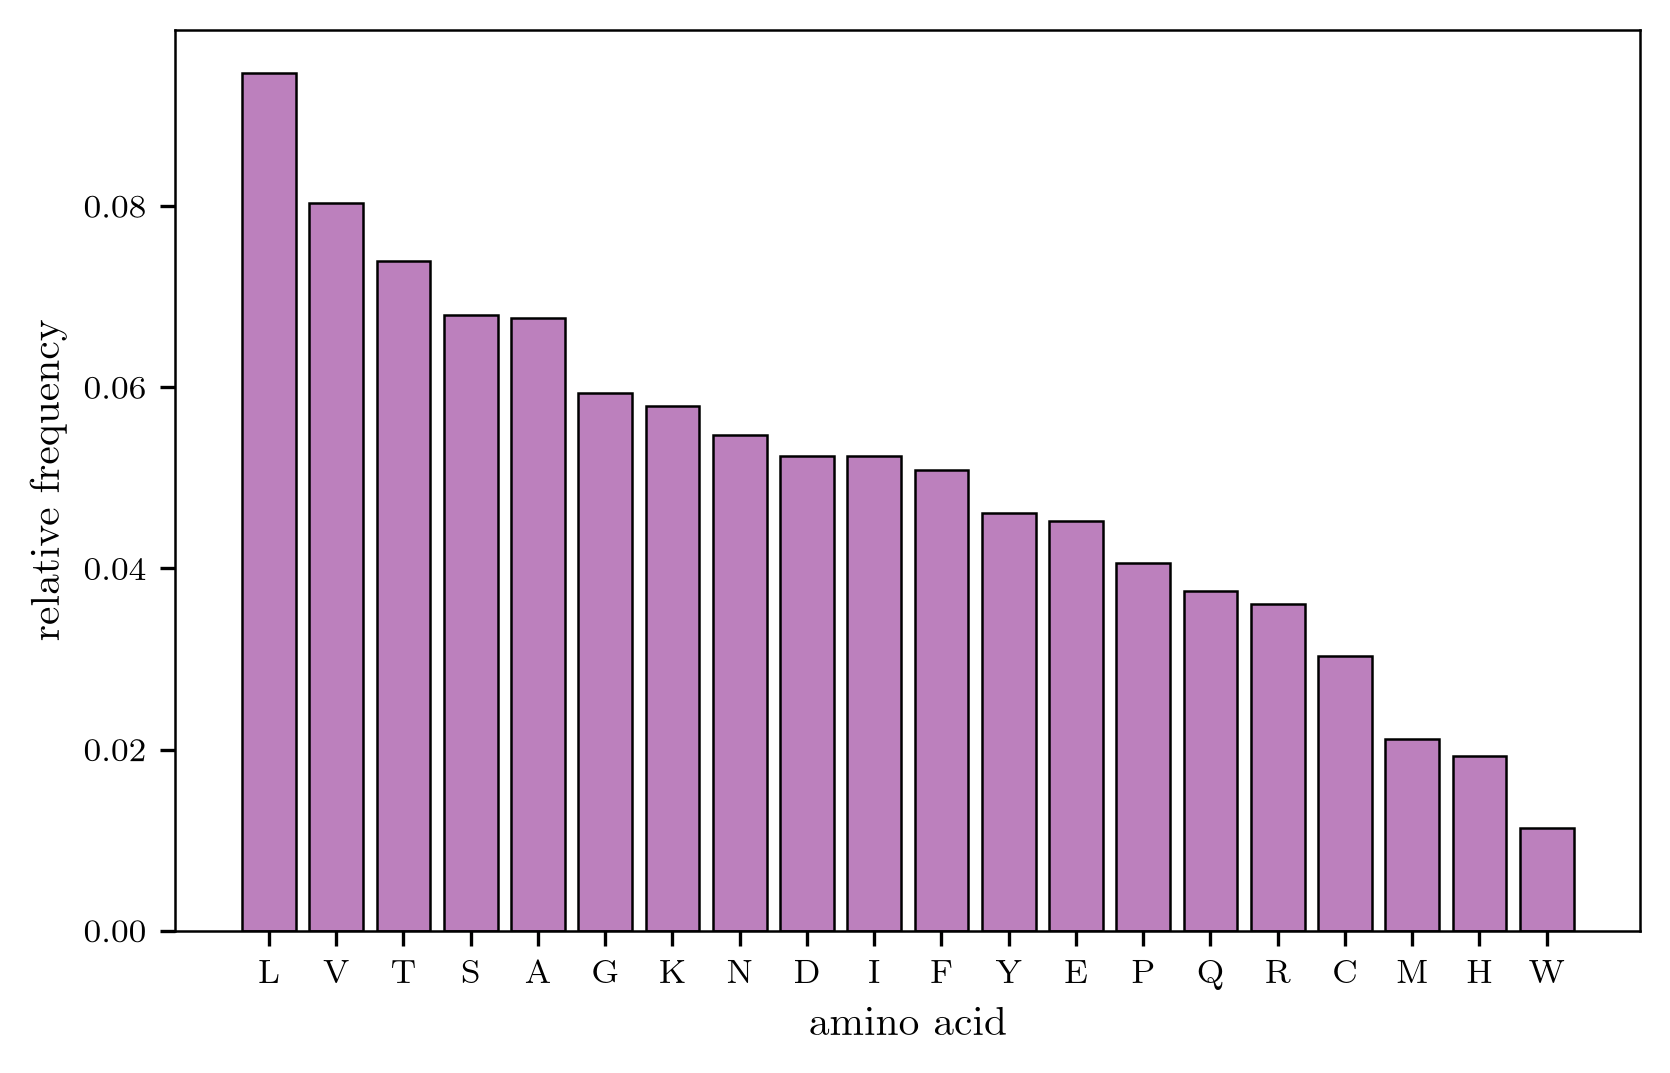
\includegraphics[width=0.7\textwidth]{fig_freq_protein}
    \caption{Pooled amino-acid frequencies over the 24 protein records.}
    \label{fig:freq_protein}
\end{figure}

\end{appendices}
